% !TEX TS-program = pdflatex
% !TEX root = ../tesi.tex


%************************************************
\chapter{Ambisonics}
\label{chp:Ambisonics}
%************************************************

Ambisonics è un formato audio surround a sfera completa: oltre al piano orizzontale, copre le sorgenti sonore sopra e sotto l'ascoltatore.
\begin{itemize}
\item Il \textbf{surround} (dal verbo inglese "to surround", in italiano "circondare", o più propriamente "avvolgere") è l'informazione sonora che in una tecnica di riproduzione/registrazione del suono (ad esempio la quadrifonia) costituisce il fronte sonoro alle spalle dell'ascoltatore.\\ Il surround, in abbinamento al fronte sonoro anteriore, ha lo scopo di collocare l'ascoltatore al centro della scena sonora, offrendo quindi la possibilità di un maggior realismo sonoro, in quanto normalmente in natura il suono raggiunge l'ascoltatore da ogni direzione.\\
\end{itemize}

\begin{figure}[h]
      \centering
      
\includegraphics[width=0.3\textwidth]{Graphics/AmbisonicLogo.png}
      \caption{⟨Logo simbolico Ambisonics⟩}
      \label{fig:⟨etichetta⟩}
      \end{figure}

\section{Premessa storica}

Michael Gerzon fece dichiarazione senza compromessi nel suo articolo intitolato
\textit{\textbf{What’s wrong with quadraphonics?}} nel Maggio del 1974 sulla rivista Studio Sound.\\
L’attacco principale che portava a questi sistemi era l’apparente localizzazione dei
suoni affidata all’immaginazione dell’ascoltatore.\\
Dopo aver catalogato i continui difetti delle registrazioni quadrifoniche, ha
continuato descrivendo un nuovo approccio alla riproduzione del suono surround,
noto come sistemi di ”\textbf{sintesi armonica}” o ”\textbf{kernel}”.\\
 Il nuovo approccio è iniziatodall’osservazione che gli effetti che si vorrebbe produrre includono un continuum
di direzioni attorno all’ascoltatore. Tali sistemi immaginano un numero
limitato di canali utilizzati per trasmettere il suono all’ascoltatore, ma sono progettati
per ricreare una gamma continua di direzioni attorno all’ascoltatore che
si avvicinano all’originale. La matematica utilizzata non è algebra ”matriciale”
(che è usata solo per descrivere trasformazioni di un numero finito di variabili)
ma algebra ”kernel” (che è la matematica corrispondente usata quando si ha un
continuum infinito di variabili).\\
Ha spiegato di essere stato recentemente associato al sistema Ambisonic, che
era un esempio di sistema kernel.\\ È stato sostenuto dalla \textbf{National Research and
Development Corporation} (\textbf{NRDC}) e ha coinvolto il professor Peter Fellgett della
Reading University.\\
Il sistema audio surround britannico Ambisonics esiste da quasi trent’anni.\\
Nonostante la mancanza del finanziamento delle principali società disponibili
per i sistemi concorrenti, Ambisonics è sopravvissuta grazie a prestazioni tecniche
superiori e al supporto di appassionati di tutto il mondo.\\
Con la facile disponibilità di una potente elaborazione del segnale digitale
 (al contrario dei circuiti analogici costosi e soggetti a errori che dovevano essere utilizzati durante i suoi primi anni)
 e il successo dell'introduzione sul mercato dei sistemi audio surround home theater sin dagli anni '90,
  l'interesse per Ambisonics tra ingegneri del suono, sound designer, compositori, società di media,
  emittenti e ricercatori è tornato e continua ad aumentare.

  \section{Introduzione}
Ambisonics può essere inteso come un'estensione tridimensionale dello stereo M/S (mid/side),
aggiungendo ulteriori canali di differenza per altezza e profondità.\\
Il set di segnali risultante è chiamato \textbf{formato B}.
I suoi canali componenti sono etichettati \textbf{W} per la pressione sonora (la M in M/S),
\textbf{X} per il gradiente di pressione sonora anteriore-meno-posteriore, 
\textbf{Y} per sinistra- meno-destra (la S in M/S) e \text{Z} per su-meno-giù. \\
Il segnale \textbf{W} corrisponde a un microfono omnidirezionale,
mentre \textbf{XYZ} sono le componenti che sarebbero captate da
capsule a forma di otto orientate lungo i tre assi spaziali.

\section{Panning di una sorgente}
Un semplice panner Ambisonic (o codificatore) prende un segnale sorgente S e due parametri,
 l'angolo orizzontale $\theta$ e l'angolo di elevazione $\phi$.\\
 Posiziona la sorgente all'angolo desiderato distribuendo il segnale sui 
 componenti Ambisonic con guadagni diversi:

 \begin{equation}
W =S\cdot\frac{1}{\sqrt{2}}
 \end{equation}

 \begin{equation}
      X=S\cdot\cos\theta\cos\phi
\end{equation}

\begin{equation}
      Y =S\cdot\sin\theta\cos\phi
\end{equation}

\begin{equation}
      Z=S\cdot\sin\phi
\end{equation}
\\

Essendo omnidirezionale, il canale W riceve sempre lo stesso segnale di ingresso costante, indipendentemente dagli angoli. \\
Affinché abbia più o meno la stessa energia media degli altri canali, W è attenuato di circa 3 dB (appunto, diviso per la radice quadrata di due).\\
 I termini per XYZ in realtà producono gli schemi polari dei microfoni a forma di otto. \\ 
 Prendiamo il loro valore $\theta$ e $\phi$ e moltiplichiamo il risultato per il segnale di ingresso.\\
  Il risultato è che l'ingresso finisce in tutti i componenti esattamente come l'avrebbe captato il microfono corrispondente.

\subsection{Microfoni virtuali}

I componenti in formato B possono essere combinati per derivare microfoni virtuali con qualsiasi diagramma polare di primo ordine (omnidirezionale, cardioide, ipercardioide, figura di otto o qualsiasi altra via di mezzo) che punta in qualsiasi direzione.
 \\È possibile derivare contemporaneamente più microfoni di questo tipo con parametri diversi, per creare coppie stereo coincidenti (come un Blumlein) o array surround.

 \begin{center}
 \captionsetup{type=table}
 \captionof{table}{Un microfono virtuale orizzontale ad angolo orizzontale $\theta$ con Pattern $0\le p\le 1$ dato da
 $M(\theta,p)=p{\sqrt{2W}}+(1-p)(\cos\theta X+\sin\theta Y)$.
 Questo microfono virtuale è normalizzato in campo libero,
  il che significa che ha un guadagno costante di uno per i suoni in asse. }
\begin{tabular}{||p{3.0cm}|p{3.0cm}||} 
      \hline\hline
      p & Pattern \\
      \hline\hline
      0 & Figura a 8 \\
      \hline\hline
      (0, 0.5) & Iper e Super-cardioide\\
      \hline\hline
      0.5 & Cardioide \\
      \hline\hline
      (0.5, 1.0) & Cardioide Largo \\
      \hline\hline
      1.0 & Omnidirezionale \\
      \hline\hline
      \end{tabular}
\end{center}

I microfoni virtuali possono essere manipolati in post-produzione: i suoni desiderati possono essere individuati,
 quelli indesiderati soppressi e l'equilibrio tra suono diretto e riverberante può essere messo a punto durante il missaggio.
 
\section{Decoding di un segnale}

Un decoder Ambisonic di base è molto simile a un set di microfoni virtuali.
Per layout perfettamente regolari, è possibile generare un decodificatore semplificato puntando un microfono cardioide virtuale in direzione di ciascun altoparlante.
\\Ecco un quadrato:

\begin{equation}
      LF = ({\sqrt{2W}} + X + Y){\sqrt{8}}
\end{equation}

\begin{equation}
      LB = ({\sqrt{2W}} - X + Y){\sqrt{8}}
\end{equation}

\begin{equation}
      RB = ({\sqrt{2W}} - X - Y){\sqrt{8}}
\end{equation}

\begin{equation}
      RF = ({\sqrt{2W}} + X - Y){\sqrt{8}}
\end{equation}

\begin{figure}[h]
      \centering
      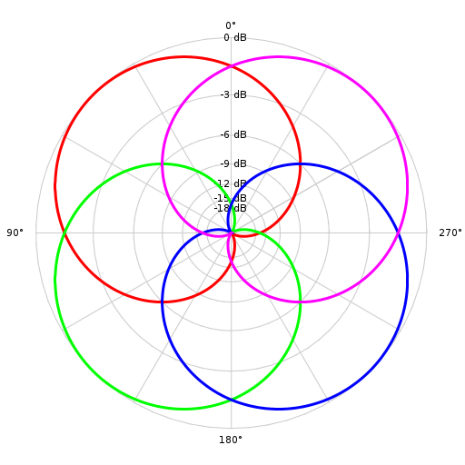
\includegraphics[width=0.8\textwidth]{Decodificatore.png}
      \caption{⟨Decodificatore basico in fase a banda singola per un layout di altoparlanti quadrati⟩}
      \label{fig:⟨etichetta⟩}
      \end{figure}

      In pratica, un vero decoder Ambisonic richiede una serie di ottimizzazioni psicoacustiche per funzionare correttamente.\\
      La decodifica dipendente dalla frequenza può anche essere utilizzata per produrre stereo binaurale;
      questo è particolarmente rilevante nelle applicazioni di realtà virtuale.
      
      \section{Gli ordini dell'Ambisonics}

      Nel contesto dei videogiochi, viene utilizzato principalmente l'ambisonics di primo ordine (o "B-format"), che consiste in quattro canali audio (W, X, Y e Z) che rappresentano rispettivamente il suono diffuso uniformemente nell'ambiente, e le tre dimensioni spaziali.\\
      Questo formato permette di ricostruire un campo sonoro 3D attraverso un numero variabile di altoparlanti, a seconda delle capacità e delle configurazioni dei sistemi di riproduzione sonora utilizzati.\\
      In genere, i videogiochi che supportano l'ambisonics di primo ordine consentono ai giocatori di selezionare il numero di altoparlanti utilizzati, in base alle loro esigenze e alle specifiche del sistema di riproduzione sonora che hanno a disposizione.\\
      Inoltre, gli sviluppatori di giochi possono utilizzare plugin o librerie di software dedicati per creare, manipolare e riprodurre il segnale ambisonico all'interno dell'ambiente di sviluppo del gioco.\\
      Il set di segnali risultante viene quindi chiamato Ambisonics di secondo, terzo o, collettivamente, di ordine superiore.\\
      Per un dato ordine $\mathbf{l}$, i sistemi a sfera completa richiedono componenti di segnale $(l+1)^{2}$ componenti, e $2l+1$ sono necessari per la riproduzione solo orizzontale.
\\
      \begin{figure}[h]
            \centering
            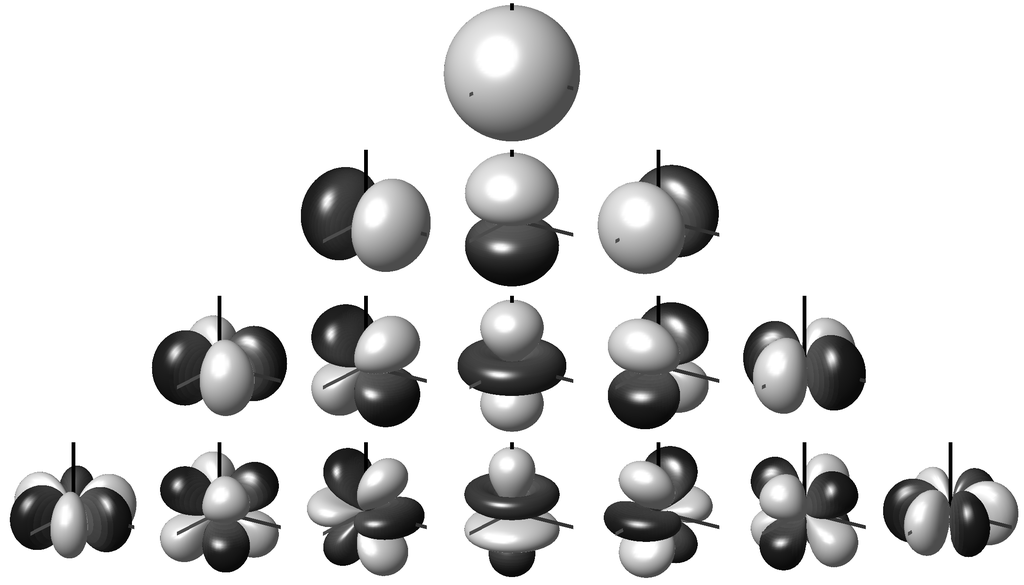
\includegraphics[width=0.8\textwidth]{OrdiniAmb.png}
            \caption{⟨Rappresentazione visiva dei componenti Ambisonic in formato B fino al terzo ordine.
            Le parti scure rappresentano le regioni in cui la polarità è invertita.
            Si noti come le prime due righe corrispondano ai modelli polari del microfono omnidirezionale e figura di otto.⟩}
            \label{fig:⟨etichetta⟩}
            \end{figure}

      \section{Problemi ed integrazioni}

      \subsection{Problemi}
      La risoluzione spaziale di Ambisonics di primo ordine come descritto sopra è piuttosto bassa.
      In pratica, ciò si traduce in sorgenti leggermente sfocate, ma anche in un'area di ascolto utilizzabile relativamente piccola o punto debole.\\
      La risoluzione può essere aumentata e lo sweet spot ampliato aggiungendo gruppi di componenti direzionali più selettivi al formato B.
      Questi non corrispondono più ai modelli polari convenzionali del microfono, ma sembrano piuttosto foglie di trifoglio. 
      
      L'utilizzo dell'Ambisonics nei videogiochi comporta alcune problematiche specifiche, tra cui:

      \begin{enumerate}
            \item Gestione del carico di lavoro del processore:
            L'elaborazione di un segnale audio in Ambisonics richiede una notevole quantità di potenza di elaborazione.
            In un videogioco, dove il processore deve gestire molte altre attività,
            questo può comportare una diminuzione delle prestazioni del gioco stesso
            
            \item Latenza: L'elaborazione in tempo reale di un segnale audio in Ambisonics può comportare un certo ritardo nella riproduzione del suono rispetto all'azione del gioco stesso.
            Questa latenza può influire sulla sensazione di immersività e può essere particolarmente problematica in giochi in cui la sincronizzazione audio-video è fondamentale.
            
\item Problemi di compatibilità: Non tutti i motori di gioco supportano l'Ambisonics, il che può limitare la sua applicazione in alcuni giochi.
Inoltre, la compatibilità con i diversi sistemi di riproduzione sonora può rappresentare una sfida per gli sviluppatori di giochi.

\item Gestione del volume: La riproduzione di un campo sonoro tridimensionale in Ambisonics comporta la gestione di più canali audio, il che può comportare difficoltà nella regolazione del volume di ogni singolo canale, soprattutto in situazioni in cui si desidera evidenziare un suono specifico o limitare il volume di altri suoni.
  
\item Codifica e decodifica: La codifica e decodifica di un segnale audio in Ambisonics richiede l'utilizzo di algoritmi specifici, che possono comportare una maggiore complessità nella produzione audio del gioco e un aumento del tempo e dei costi di sviluppo.

\end{enumerate}

\subsection{integrazioni}

Nonostante la limita disponibilità dei software e degli hardware disponibili per l'utilizzo di Ambisonics all'interno
dei videogiochi, esistono degli sviluppatori che hanno segnato una loro impronta storica in questo ambito sonoro:

\begin{enumerate}
      \item Unity: Unity è uno dei motori di gioco più popolari ed è ampiamente utilizzato per la produzione di giochi per molte piattaforme. Supporta l'Ambisonics attraverso plugin di terze parti come Facebook 360 Spatial Workstation e Steam Audio.
      \item Unreal Engine: Unreal Engine è un altro motore di gioco molto popolare, utilizzato per la produzione di molti giochi di successo. Supporta l'Ambisonics attraverso il plugin Steam Audio.
      \item FMOD Studio: FMOD Studio è un motore audio utilizzato per la produzione di suoni in giochi, film e altri progetti multimediali. Supporta l'Ambisonics attraverso il suo plugin Spatializer.
      \item Wwise: Wwise è un altro motore audio utilizzato per la produzione di suoni in giochi e altri progetti multimediali. Supporta l'Ambisonics attraverso il plugin Spatial Audio.
\end{enumerate}
